
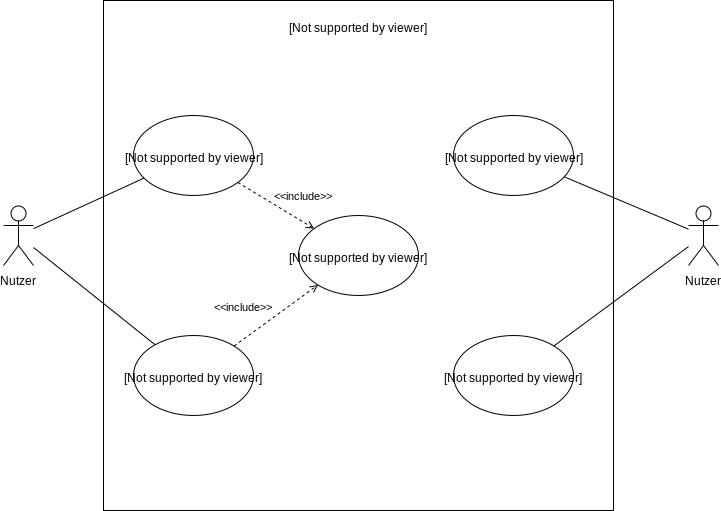
\includepdf[pages=-, scale=0.8, pagecommand={\subsection{Anwendungsfälle}\subsubsection{Client}Anwendungsfälle der Client-Anwendung. Der Anwendungsfall \glqq{}Spiel spielen\grqq{} wird unter \ref{ssec:Partie}~ konkretisiert. Hinweis: Der zweite Akteur wurde nur aus Übersichtlichkeitsgründen hinzugefügt und stellt keinen zweiten Nutzer dar.}]{../Meilenstein02/images/AFD_Client.pdf}

\includepdf[pages=-, scale=0.8, pagecommand={\subsubsection{KI-Client}Anwendungsfälle des KI-Clients. Diese Anwendung verbindet sich mit einem Server und simuliert mithilfe einer zuvor konfigurierten KI einen menschlichen Gegenspieler. Der Anwendungsfall \glqq{}Spiel spielen\grqq{} wird unter \ref{ssec:Partie}~ konkretisiert.}]{../Meilenstein02/images/AFD_KIClient.pdf}

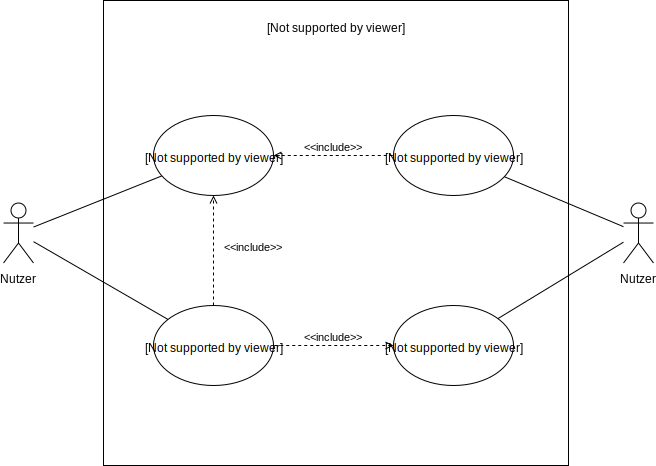
\includepdf[pages=-, scale=0.8, pagecommand={\subsubsection{Editor}Anwendungsfälle der Editor-Anwendung. Der zweite Akteur wurde nur aus Übersichtlichkeitsgründen hinzugefügt und stellt keinen zweiten Nutzer dar.}]{../Meilenstein02/images/AFD_Editor.pdf}
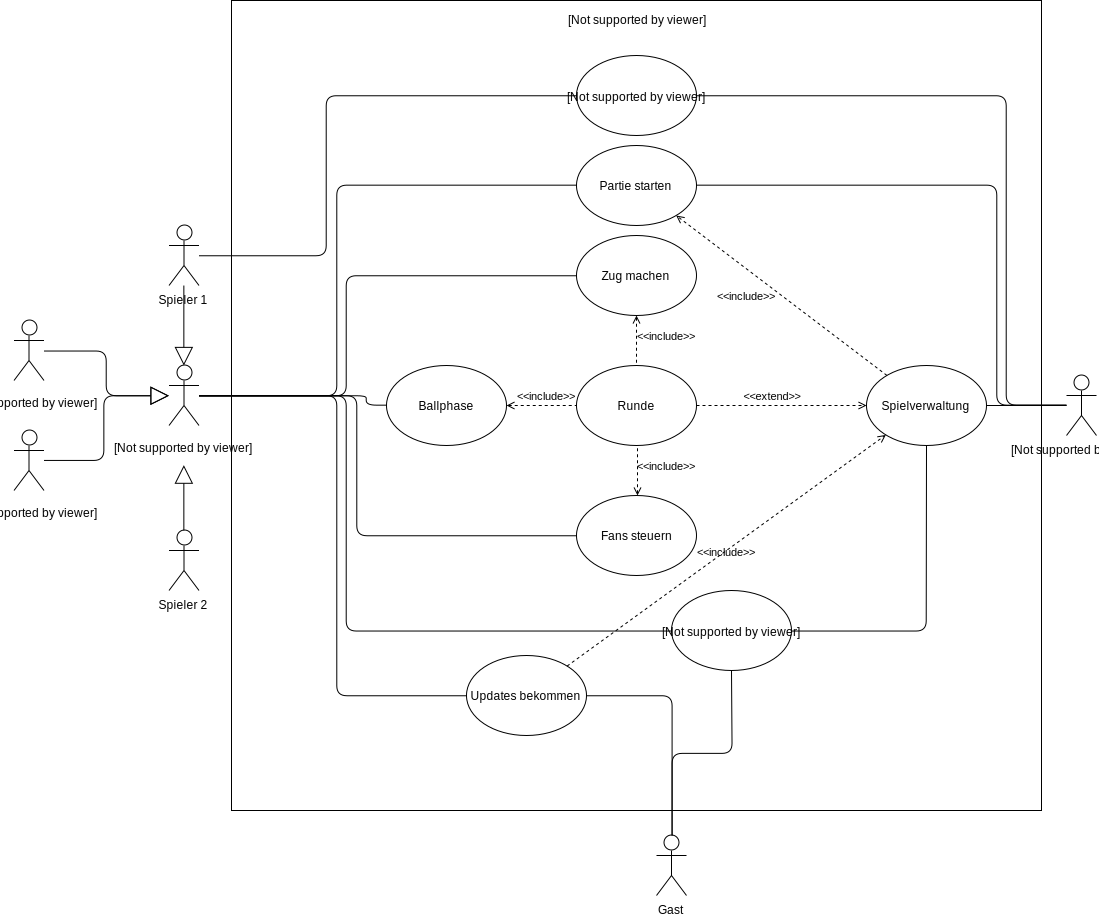
\includepdf[pages=-, scale=0.8, pagecommand={\subsubsection{Partie}\label{ssec:Partie}Mögliche Anwendungsfälle, die während einer Partie auftreten. Die Runde stellt einen abstrakten Anwendungsfall dar, der sich aus den einzelenen Phasen einer Runde zusammensetzt.}]{../Meilenstein02/images/AFD_Party.pdf}


\subsection{Zuordnung der Anforderungenn zu Anwendungsfällen}
\subsubsection{Hauptmenü öffnen}
\begin{itemize} 
	\item FA60
\end{itemize}
\subsubsection{Hilfe anzeigen}
\begin{itemize} 
	\item FA65
\end{itemize}
\subsubsection{Spielende-Bildschirm}
\begin{itemize} 
	\item FA49
	\item FA62
\end{itemize}
\subsubsection{Spiel visualisieren}
\begin{itemize} 
	\item FA1
	\item FA2 
	\item FA3 
	\item FA4 
	\item FA5 
	\item FA6 
	\item FA64 
\end{itemize}
\subsubsection{Spiel beobachten}
\begin{itemize} 
	\item FA55
	\item FA66 
\end{itemize}
\subsubsection{Spiel beitreten}
\begin{itemize} 
	\item FA55
	\item FA61 
\end{itemize}
\subsubsection{Spiel spielen}
\begin{itemize} 
	\item FA14 
	\item FA15 
	\item FA16 
	\item FA17 
	\item FA18 
	\item FA19 
	\item FA20 
	\item FA55 
	\item FA67
	\item FA68 
	\item FA69 
\end{itemize}
\subsubsection{Schwierigkeit einstellen}
\begin{itemize} 
	\item FA73 
\end{itemize}
\subsubsection{Serverkonfiguration einstellen}
\begin{itemize} 
	\item FA74 
\end{itemize}
\subsubsection{Team-Konfiguration laden}
\begin{itemize} 
	\item FA75 
\end{itemize}
\subsubsection{Konfiguration erstellen}
\begin{itemize} 
	\item FA14
	\item FA15 
	\item FA53 
	\item FA54 
	\item FA71 
\end{itemize}
\subsubsection{Konfiguration speichern}
\begin{itemize} 
	\item FA14
	\item FA15 
	\item FA53 
	\item FA54 
	\item FA71 
\end{itemize}
\subsubsection{Konfiguration bearbeiten}
\begin{itemize} 
	\item FA14
	\item FA15 
	\item FA53 
	\item FA54 
	\item FA70 
	\item FA72 
\end{itemize}
\subsubsection{Konfiguration öffnen}
\begin{itemize} 
	\item FA14
	\item FA15 
	\item FA53 
	\item FA54 
	\item FA63 
\end{itemize}
\subsubsection{Team-Konfiguration laden}
\begin{itemize} 
	\item FA14
	\item FA15 
	\item FA54 
	\item FA55 
	\item FA63 
\end{itemize}
\subsubsection{Partie starten}
\begin{itemize} 
	\item FA50
	\item FA51 
	\item FA55 
\end{itemize}
\subsubsection{Zug machen}
\begin{itemize} 
	\item FA8
	\item FA21 
	\item FA22 
	\item FA24 
	\item FA26 
	\item FA27 
	\item FA28 
	\item FA29 
	\item FA30 
	\item FA37 
	\item FA38 
	\item FA39 
	\item FA40 
	\item FA41 
	\item FA42 
	\item FA46 
	\item FA55 
\end{itemize}
\subsubsection{Runde}
\begin{itemize} 
	\item FA10
	\item FA11 
	\item FA12 
	\item FA13 
	\item FA25 
	\item FA44 
	\item FA55 
\end{itemize}
\subsubsection{Ballphase}
\begin{itemize} 
	\item FA10
	\item FA11 
	\item FA12 
	\item FA13 
	\item FA29 
	\item FA45 
	\item FA55 
\end{itemize}
\subsubsection{Fans steuern}
\begin{itemize} 
	\item FA31
	\item FA32 
	\item FA33 
	\item FA34 
	\item FA35 
	\item FA47 
	\item FA55 
\end{itemize}
\subsubsection{Spielverwaltung}
\begin{itemize} 
	\item FA1
	\item FA2 
	\item FA3 
	\item FA4 
	\item FA5 
	\item FA6 
	\item FA7 
	\item FA9 
	\item FA23 
	\item FA30 
	\item FA36 
	\item FA43 
	\item FA48 
	\item FA49 
	\item FA52 
	\item FA53 
	\item FA54 
	\item FA56 
	\item FA58 
	\item FA59 
\end{itemize}
\subsubsection{Updates bekommen}
\begin{itemize} 
	\item FA55
\end{itemize}
\subsubsection{Zu Partie anmelden}
\begin{itemize} 
	\item FA55
\end{itemize}
\subsubsection{Partie-Konfiguration laden}
\begin{itemize} 
	\item FA53
	\item FA57
\end{itemize}

\includepdf[pages=-, scale=0.8, pagecommand={\subsection{Abläufe im System}\subsubsection{State-Machine Clientanwendung} Zustandsdiagramm für die verschiedenen Ansichten der Client-Anwendung.}]{../Meilenstein02/images/Client_SM.pdf}

\includepdf[pages=-, scale=0.8, pagecommand={\subsubsection{State-Machine Partie Server} Zustandsdiagramm des Servers für eine komplette Partie, inklusive Anmeldung der Spieler und eventuelle Verbindungsabbrüche.}]{../Meilenstein02/images/SM_Server.pdf}

\includepdf[pages=-, scale=0.9, pagecommand={\subsubsection{State-Machine Partie Client}Zustandsdiagramm der Client-Anwendung für eine komplette Partie.}]{../Meilenstein02/images/SM_ClientAnmelden.pdf}

\includepdf[pages=-, scale=0.8, pagecommand={\subsubsection{Sequenzdiagramm Spielaufstellung}Kommunikation zwischen Spieler und Server während der Spielaufstellungsphase.}]{../Meilenstein02/images/SD_Spielaufstellung.pdf}

\includepdf[pages=-, scale=0.8, pagecommand={\subsubsection{Sequenzdiagramm Spielvorbereitung}Nachrichtenaustausch zwischen Server und den Spielern während der Vorbereitung auf die Partie.}]{../Meilenstein02/images/SD_Spielvorbereitung.pdf}
\includepdf[pages=-, scale=0.8, pagecommand={\subsubsection{State-Machine Rundenablauf}Ablauf der Spielphasen im Spiel}]{../Meilenstein02/images/SM_Rundenablauf.pdf}
\includepdf[pages=-, scale=0.8, pagecommand={\subsubsection{Sequenzdiagramm Ballphase}}]{../Meilenstein02/images/SD_Ballphase.pdf}
\includepdf[pages=-, scale=0.65, pagecommand={\subsubsection{Sequenzdiagramm Spielerphase}}]{../Meilenstein02/images/SD_Spielerphase.pdf}
\includepdf[pages=-, scale=0.8, pagecommand={\subsubsection{Sequenzdiagramm Fanphase}}]{../Meilenstein02/images/SD_Fanphase.pdf}
\includepdf[pages=-, scale=0.7, pagecommand={\subsubsection{State-Machine Überlängenbehandlung}}]{../Meilenstein02/images/SM_Ueberlaenge.pdf}
\includepdf[pages=-, scale=0.7, pagecommand={\subsubsection{Sequenzdiagramm Gast}}]{../Meilenstein02/images/SD_Gast.pdf}
